\documentclass[utf8x,notes=hide]{beamer}
\mode<article>
{
  \usepackage{fullpage}
  \usepackage{pgf}
  \usepackage{hyperref}
  \setjobnamebeamerversion{beamer}
}

\mode<presentation>
{
  %\usetheme{Frankfurt}
 %\usetheme{My}
  \usetheme{Madrid}
  % or ...
%\usecolortheme{seagull}
  %\setbeamercovered{transparent}
  %\setbeamercovered{dynamic}
  % or whatever (possibly just delete it)
}
\usenavigationsymbolstemplate{}
\usefonttheme{structurebold}
\usepackage{multimedia}
\usepackage{tikz}
\usepackage{fontspec,xunicode,xltxtra}
%\usepackage[scaled=.90]{helvet}
% Or whatever. Note that the encoding and the font should match. If T1
% does not look nice, try deleting the line with the fontenc.

\setbeamertemplate{footline}
{
\leavevmode
%\hbox{\begin{beamercolorbox}[wd=.5\paperwidth,ht=2.5ex,dp=1.125ex,
%leftskip=.3cm plus1fill,rightskip=.3cm]{author in head/foot}%
%    \usebeamerfont{author in head/foot}\insertshortauthor
%  \end{beamercolorbox}%
%  \begin{beamercolorbox}[wd=.5\paperwidth,ht=2.5ex,dp=1.125ex,leftskip=.3cm,
%rightskip=.3cm plus1fil]{title in head/foot}%
%    \usebeamerfont{title in head/foot}\insertshorttitle\hfill

\hfill\insertframenumber  \hspace{3pt}

%\inserttotalframenumber
%\hspace*{2ex}
%  \end{beamercolorbox}}%
  \vskip3pt%
}

%\usepackage[english]{babel}
\usepackage[ngerman]{babel}
\selectlanguage{ngerman}

%
% math/symbols
%
\usepackage{amssymb}
\usepackage{amsthm}
% \usepackage{latexsym}
\usepackage{amsmath}
%\usepackage{listings}
\usepackage[framed]{mcode}
%\usepackage{mcode}

\usepackage{mydef}
\usepackage{cmap} % you can search in the pdf for umlauts and ligatures
%\usepackage{colonequals} %corrects the definition-symbols \colonequals (besides others)
\title{Einführung in Matlab}
%
%\subtitle{Disputation} % (optional)

\author{Jochen Schulz}
% - Use the \inst{?} command only if the authors have different
%   affiliation.

\institute{Georg-August Universit\"at G\"ottingen \pgfimage[height=0.5cm]{../figures/unilogo3}}
% - Use the \inst command only if there are several affiliations.
% - Keep it simple, no one is interested in your street address.

\date{\today}

\subject{Einführung in Matlab}
% This is only inserted into the PDF information catalog. Can be left
% out. 



% If you have a file called "university-logo-filename.xxx", where xxx
% is a graphic format that can be processed by latex or pdflatex,
% resp., then you can add a logo as follows:

%\logo{\pgfimage[height=0.5cm]{figures/unilogo3}}


% Delete this, if you do not want the table of contents to pop up at
% the beginning of each subsection:
% \AtBeginSubsection[]
% {
%   \begin{frame}<beamer>
%     \frametitle{Aufbau}
%     \tableofcontents[currentsection,currentsubsection]
%   \end{frame}
% }

\AtBeginSection[]
{
  \begin{frame}<beamer>
    \frametitle{Aufbau}
    \tableofcontents[currentsection,currentsubsection]
  \end{frame}
}


\begin{document}



\subtitle{Einheit 3 \\ Grafik, Arbeiten mit Polynomen }


\begin{frame}[fragile]
  \titlepage
\note{}
\end{frame}

\begin{frame}[fragile]
  \frametitle{Aufbau}
  \tableofcontents
\note{}
  % You might wish to add the option [pausesections]
\end{frame}



\section{Einf\"uhrung Grafik}
\subsection{einfache zweidimensionale Grafiken}
% 
% Slide
% 
\begin{frame}[fragile]\frametitle{Standard-Plot}
\begin{lstlisting}
plot(x,y)
\end{lstlisting}
zeichnet für Vektoren $x=(x_1, \ \dots \ ,x_N)$ und  $y=(y_1, \dots \ ,y_N)$
eine Grafik, die die Punkte $(x_i,y_i)$ und $(x_{i+1},y_{i+1})$ miteinander
verbindet.

\begin{columns}[c]
 \column{0.4\textwidth}
\begin{lstlisting}
>> x=linspace(0,2*pi,100);
>> y1=sin(3*x);
>> plot(x,y1)
\end{lstlisting}
 \column{0.55\textwidth}
\pgfimage[width=0.9\textwidth]{./../figures/grafik_1}
\end{columns}
\end{frame}
% 
% Slide
% 
\begin{frame}[fragile]\frametitle{Erweiterungen}
\begin{lstlisting}
plot(x,y,string)
\end{lstlisting}
\alert{String} besteht aus drei Elementen, die die Farbe, Linienstil
und die Markierung der Punkte kontrollieren. Die Reihenfolge der drei
Elemente ist beliebig.
\begin{columns}[c]
 \column{0.4\textwidth}
{\it Beispiel:} Durch \\
\alert{ \lstinline!plot(x,y,'r*--')!} wird die Linie
gestrichelt (- -) in rot (r) gezeichnet und die Punkte durch *
markiert.
\column{0.55\textwidth}
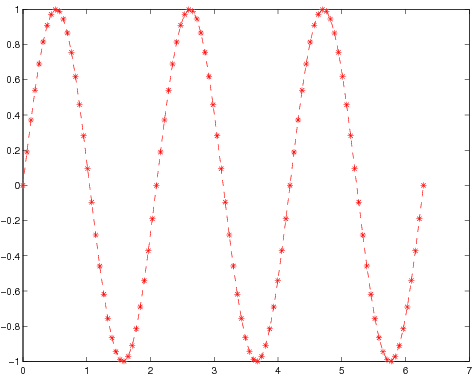
\includegraphics[width=\textwidth]{./../figures/grafik_2}
\end{columns}
\end{frame}
% 
% Slide
% 
\begin{frame}[fragile]\frametitle{Optionen}
\begin{tabular}{cp{8.5cm}}
\alert{ Farben} & r (rot), g (grün), b (blau), c (hellblau), m (magenta),
  y (gelb), k (schwarz), w (weiß)\\
\alert{ Marker} & o (Kreis), * (Stern), . (Punkt), + (Plus), x (Kreuz), s
  (Quadrat), d (Raute),... \\
\alert{ Linien-Stil} &  - (durchgezogene Linie), \lstinline!--! (gestrichelte
  Linie), \lstinline!:! (gepunktete Linie), \lstinline!-.! (Strich-Punkt Linie)\\
\end{tabular}

Läßt man den Linien-Stil weg, so werden die Punkte nicht verbunden.
\end{frame}

% 
% Slide
% 
\begin{frame}[fragile]\frametitle{Optionen II}
\begin{lstlisting}
plot(x,y,string,Eigenschaft, Spez.) 
\end{lstlisting}
\alert{ Eigenschaften:}\\
\lstinline!'MarkerSize'! (Default 6), \lstinline!'LineWidth'! (Default 0.5),
\lstinline!'MarkerEdgeColor'!, \lstinline!'MarkerFaceColor'!\\

\begin{columns}[c]
 \column{0.55\textwidth}
{\it Beispiel:} \\
\begin{lstlisting}
>>plot(x,y1,'b-.d','LineWidth',3,...
'MarkerEdgeColor','g')
\end{lstlisting}
\column{0.45\textwidth}
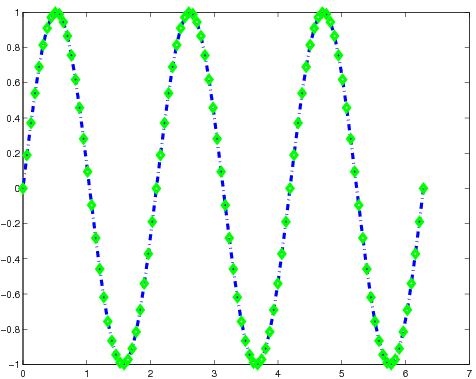
\includegraphics[width=\textwidth]{./../figures/grafik_3}
\end{columns}
\end{frame}
% 
% Slide
% 
\begin{frame}[fragile]\frametitle{Alternativen}
\begin{itemize}
\item Mehrere Plots in eine Grafik:
\alert{ \lstinline!plot(x1,y1,string1,x2,y2,string2,...)!}
\item Logaritmische Skalierung in $x$- bzw in $y$-Richtung: \alert{ \lstinline!semilogx(x1,y1)!} bzw. \alert{
  \lstinline!semilogy(x1,y1)!}.
\item Logarithmische Skalierung beider Achsen: \alert{
  \lstinline!loglog(x1,y1)!}   
\item Ist $X$ ein Vektor mit komplexen Einträgen, so ergibt \alert{
  \lstinline!plot(X)!} \lstinline!plot(real(X),imag(X))!.
\end{itemize}
\end{frame}
% 
% Slide
% 
\begin{frame}[fragile]\frametitle{Beispiel - Legendre Polynome}
%\begin{columns}[c]
% \column{0.52\textwidth}
\begin{lstlisting}[basicstyle=\scriptsize]
>> x=linspace(-1,1,100);
>> p1=x;
>> p2=(3/2)*x.^2-1/2;
>> p3=(5/2)*x.^3-(3/2)*x;
>> p4=(35/8)*x.^4 - (15/4)*x.^2+3/8;
>> plot(x,p1,'r:',x,p2,'g--',x,p3,'b-.',x,p4,'m-','LineWidth',2)
\end{lstlisting}
%\column{0.48\textwidth}
\hfil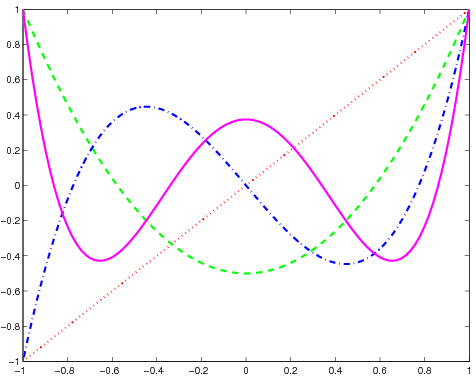
\includegraphics[width=0.55\textwidth]{./../figures/grafik_4}\hfil
%\end{columns}
\end{frame}
% 
% Slide
% 
\begin{frame}[fragile]\frametitle{Achseneinstellungen}
\begin{tabular}{p{3cm}p{8cm}}
\lstinline!axis([x1 x2 y1 y2])! & Setzen der $x$- und $y$-Achsen
Grenzen\\
\lstinline!axis auto! & Rückkehr zu Default Achsen Grenzen\\
\lstinline!axis equal! & Gleiche Dateneinheiten auf allen Achsen\\
\lstinline!axis off! & Enfernen der Achsen\\
\lstinline!axis square! & quadratische Achsen-Box\\
\lstinline!axis tight! & Achsen Grenzen werden passend zu den Daten
gewählt. \\
\lstinline!xlim([x1 x2])! & Setzen der $x$-Achse\\
\lstinline!ylim([y1 y2])! & Setzen der $y$-Achse\\
\lstinline!grid on! & Gitter aktivieren\\
\lstinline!box on!, \lstinline!box off!  & Box um die Grafik
legen, Box entfernen
\end{tabular}
\end{frame}
%
% Folie
%
\begin{frame}[fragile]\frametitle{Exkurs: Characters (char)}
\alert{Characters:} \\
Characters (Zeichen) sind einzelne
Zeichen. \\

Intern werden Characters in MATLAB durch Integer dargestellt. Die Werte zwischen 0 und
128 entsprechen den ASCII Werten. Insgesamt wird zur Speicherung eines Zeichens 2
Bytes ben\"otigt. Es wird also jedem Zeichen eine Zahl zwischen 0 und $2^{16}-1$
zugeordnet. 
\begin{lstlisting}
> s='d'
s =
d
>> s1=double(s)
s1 =
   100
>> s2=char(100)
s2 =
d
\end{lstlisting}
\end{frame}
%
% Folie
%
\begin{frame}[fragile]\frametitle{Exkurs: Strings}

\alert{String:}\\
 Ein String ist ein Vektor von character (Zeichen). Intern werden sie
 durch die ASCII Werte dargestellt. 
\begin{lstlisting}
>> s='AB6de*'
s =
AB6de*
>> sd=double(s)
sd =
    65    66    54   100   101    42
>> s2=char(sd)
s2 =
AB6de*
\end{lstlisting}  
\end{frame}
%
% Folie
%
\begin{frame}[fragile]\frametitle{Exkurs: Befehle für Strings}
\begin{itemize}
\item Durch \lstinline!strcat! werden Strings verbunden, z.B. \lstinline!strcat('Hello',' world')!. 
%\begin{lstlisting}
%>> strcat('Hello',' world')
%ans =
%Hello world
%\end{lstlisting}
\item \lstinline!num2str(x,n)! konvertiert $x$ in einen String mit $n$
  signifikanten Stellen. (Default: $n=4$)
\item \lstinline!int2str(x)! rundet $x$ und konvertiert es in einen String.
\item \lstinline!strcmp(s,t)! vergleicht die Strings $s$ und $t$. 
\item Durch \lstinline!help strfun! erhält man eine Liste aller Befehle im
  Zusammenhang mit Strings.
\end{itemize}
\end{frame}

\subsection{Beschriftungen}
% 
% Slide
% 
\begin{frame}[fragile]\frametitle{Beschriften der Grafik}
\begin{itemize}
\item Titel:  \alert{ \lstinline!title('Titel')!}
\item Achsenbeschriftung:  \alert{ \lstinline!xlabel('Text')!},
  \alert{ \lstinline!ylabel('Text')!} 
\item Legende: \alert{ \lstinline!legend('Text1','Text2',...,nr)!} \\
{\scriptsize \alert{ nr} gibt die Position der Legendenbox in der Grafik an:
  -1 (rechts vom Plot), 0 'bester' Ort, 1 oben rechts (default), 2
  oben links, 3 unten links, 4 unten rechts. }
\item zusätzlicher Text: \alert{ \lstinline!text(x,y,'Text')!} Plaziert
  'Text' an die Position $(x,y)$ bzgl. der Werte auf der $x$-
  bzw. $y$-Achse. 
\end{itemize}
\end{frame}
% 
% Slide
% 
\begin{frame}[fragile]\frametitle{Bemerkungen zur Beschriftung}
\begin{itemize}
\item  In den strings kann \LaTeX-Notation verwendet werden: \\
Beispiele: 
\begin{itemize} \item \lstinline!\alpha! $\Rightarrow$ $\alpha$
\item \lstinline!sin^{3/2}(x)! $\Rightarrow$ $\sin^{3/2}(x)$ . 
\end{itemize}
\item Ändern der Schriftgröße, z.B. \lstinline!title('Titel','FontSize', 20)!.
\item Auflistung aller modifizierbaren Texteigenschaften: \lstinline!doc text_props!
\end{itemize}
\end{frame}
% 
% Slide
% 
\begin{frame}[fragile]\frametitle{Beispiel - Legendre Polynome II}
\begin{lstlisting}[basicstyle=\scriptsize]
>> title('Legendre Polynome','FontSize', 20)
>> xlabel('x','FontSize', 20)
>> text(0,0.45,'Maximum')
>> legend('n=1','n=2','n=3','n=4',4)
>> grid on, box on;
>> xlim([-1.1,1.1])
\end{lstlisting}
\hfil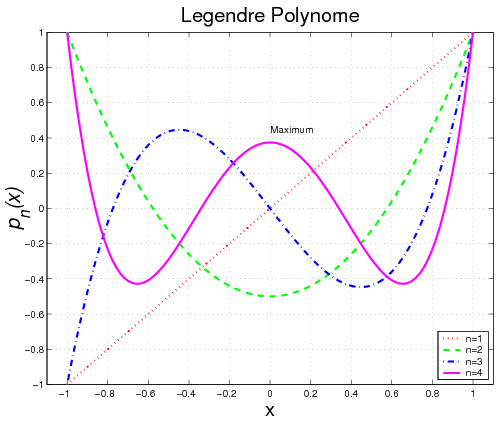
\includegraphics[width=0.5\textwidth]{./../figures/grafik_5}\hfil
%\end{columns}
\end{frame}
% 
% Slide
% 
\begin{frame}[fragile]\frametitle{Umgang mit Grafikfenster}
\begin{itemize}
\item Öffnen eines (weiteren) Grafikfensters: \lstinline!figure!.  Eine
  Grafik wird immer im aktuellen Fenster erzeugt. Ist noch kein
  Fenster geöffnet, so wird ein Fenster erzeugt.
\item Durch den Befehl \lstinline!hold on! werden bestehende Grafiken im
  aktuellen Fenster erhalten. Neue Grafiken werden den bestehenden
  hinzugefügt. 
\item \lstinline!hold off! (default) überschreibt Grafiken im
  aktuellen Fenster
\item Schliessen: \lstinline!close!, \lstinline!close all!
\end{itemize}
\end{frame}

\subsection{Anwendung: polynomiale Interpolation}
% 
% Slide
% 
\begin{frame}[fragile]\frametitle{Polynomiale Interpolation}
\begin{columns}[b]
 \column{0.6\textwidth}
Suche ein Polynom vom Grad 3
\[ p(x)= p_0 +p_1 x +p_2 x^2 +p_3 x^3,  \]
 dass durch die vier Punkte
$(0,1)$, $(1,1)$, $(2,4)$, $(5,3)$
verläuft.
\column{0.4\textwidth}
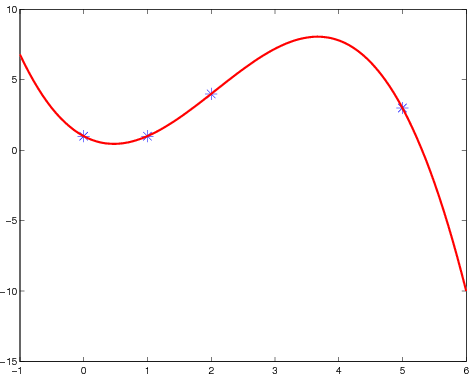
\includegraphics[width=\textwidth]{./../figures/grafik_6}
\end{columns}
$\Rightarrow  \alert{ p(0)=1, \ p(1)=1, \ p(2)=4, \ p(5)=3}$

$\Rightarrow \quad$ Lineares GLS \alert{ $Ap=b$} mit
{\scriptsize \[ A= \left( \begin{array}{cccc}
1 & 0 & 0 & 0\\
1 & 1 & 1 & 1\\
1 & 2 & 2^2 & 2^3 \\
1 & 5 & 5^2 & 5^3 \\
\end{array} \right), \
p=\left( \begin{array}{c} 
p_0 \\ p_1 \\ p_2 \\p_3\\
\end{array} \right),
\
b=\left( \begin{array}{c} 
1 \\ 1 \\ 4 \\ 3\\
\end{array} \right),
\]}  
\end{frame}
% 
% Slide
% 
\begin{frame}[fragile]\frametitle{Polynomiale Interpolation II}
Suche ein Polynom vom Grad n
\[ p(x)= p_0 +p_1 x +p_2 x^2 +p_3 x^3+ \dots +p_n x^n,  \]
 dass durch die  $n+1$ Punkte $(x_i,y_i)_{i=0}^n$
verläuft.\\[1cm]

\textbf{Beispiel}: Interpolation von
\[ (x_i,y_i)_{i=0}^{12} \]
mit \lstinline!x=linspace(-5,5,13)! und $y_i=\frac{1}{1+x_i^2}$. 
\end{frame}
% 
% Slide
% 
\begin{frame}[fragile]\frametitle{Polynomiale Interp.: Beispiel}
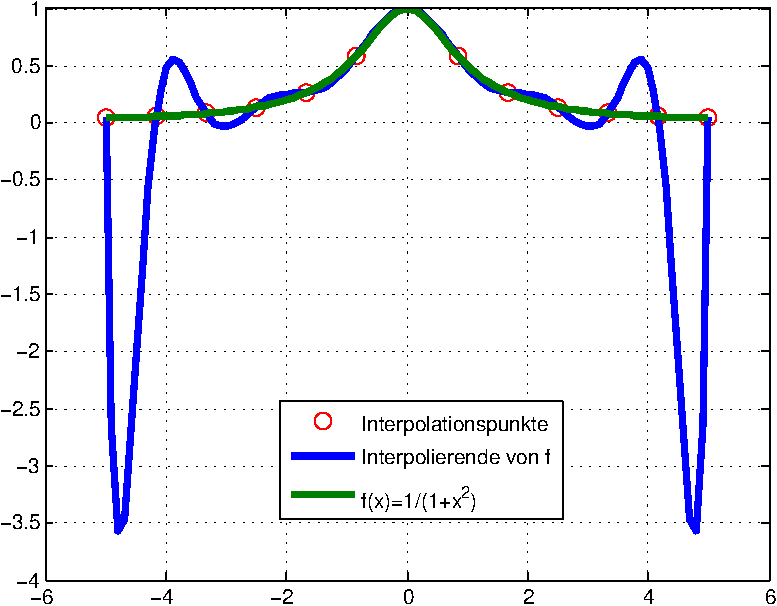
\includegraphics[width=\linewidth]{./../figures/grafik_7}
\end{frame}
% 
% Slide
% 
\begin{frame}[fragile]\frametitle{Programm 1}
\begin{lstlisting}
function p=interpol2(x,y)
% interpol2 berechnet zu n+1 Punkten (x_i,y_i)
%           das Polynom n-ten Grades, das durch die
%           n+1 Punkte verlaeuft
%           INPUT: Vektoren x,y
%           OUTPUT: Koeffizientenvektor p
%   Gerd Rapin    23.11.2003

% Aufstellen des lin. GLS
A = vandermonde(x);

% Loesen des lin GLS
p = A\y';
\end{lstlisting}
\end{frame}
% 
% Slide
% 
\begin{frame}[fragile]\frametitle{Programm 2}
\begin{lstlisting}
%---------------------------
%      interpol3.m
%  berechnet die polynomiale
%  Interpolation fuer 1/(1+x^2)
%   Gerd Rapin  23.11.2003
%--------------------------------
x = linspace(-5,5,13); % Stuetzstellen
y = 1./(1+x.*x);
plot(x,y,'or','Markersize',8); hold on;
p = interpol2(x,y); % Berechnen der Koeffizienten
x1 = linspace(-5,5,100);
y1 = ausw_poly2(p',x1);
y2 = 1./(1+x1.*x1);
plot(x1,y1,x1,y2,'Linewidth',3);
xlim([-6,6]); grid on; box on;
legend('Interpolationspunkte','Interpolierende von f',...
 'f(x)=1/(1+x^2)');
\end{lstlisting}
\end{frame}

\subsection{Weitere zweidimensionale Darstellungsmöglichkeiten}

% 
% Slide
% 
\begin{frame}[fragile]\frametitle{Darstellung von Daten}
\begin{minipage}{3cm}
Daten: 
\end{minipage}
\begin{minipage}{7cm}
\begin{lstlisting}
>> n=linspace(0,10,40);
>> y=n.^2.*exp(-n);
\end{lstlisting}
\end{minipage}\\
\begin{itemize}
\item Balkendiagramm: \alert{ \lstinline!bar(y)!}
\item Histogramm: \alert{ \lstinline!hist(y,5)!}
\item einfacher Plot: \alert{ \lstinline!area(n,[y',2*y'])!}
\item Tortengrafik:  \alert{ \lstinline!pie3([ 1 2 3 4])!}
\end{itemize}
\end{frame}
% 
% Slide
% 
\begin{frame}[fragile]\frametitle{Darstellung von Daten}
\begin{center}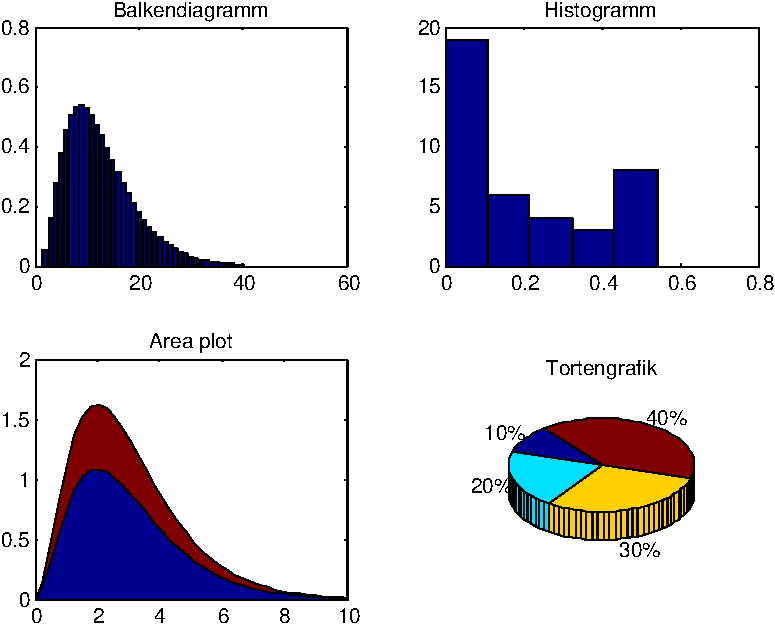
\includegraphics[height=0.8\textheight]{./../figures/darstellung_daten_2d}\end{center}
\end{frame}
% 
% Slide
% 
\begin{frame}[fragile]\frametitle{Darstellung von Daten}
\begin{lstlisting}
n = linspace(0,10,40);
y = n.^2.*exp(-n);

% Balkendiagramm
subplot(2,2,1),
bar(y); title('Balkendiagramm');

% Histogramm
subplot(2,2,2),
hist(y,5); title('Histogramm');

% Area plot
subplot(2,2,3),
area(n,[y',2*y']); title('Area plot');

% Tortengrafik
subplot(2,2,4),
pie3([ 1 2 3 4]); title('Tortengrafik');
\end{lstlisting}
\end{frame}
% 
% Slide
% 
\begin{frame}[fragile]\frametitle{Approximation von Integralen}
Approximiere $\int_0^1 f(x) dx$ durch
{\tiny \[ \int_0^1 f(x) dx \approx  \sum_{i=1}^{N} \frac{1}{N} f \left(
\frac{i-\frac{1}{2}}{N} \right ) \]}
für gegebenes $N \in \mathbb{N}$. \textbf{Beispiel}: $f(x)=x^3$
\begin{columns}[t]
\column{0.5\textwidth}
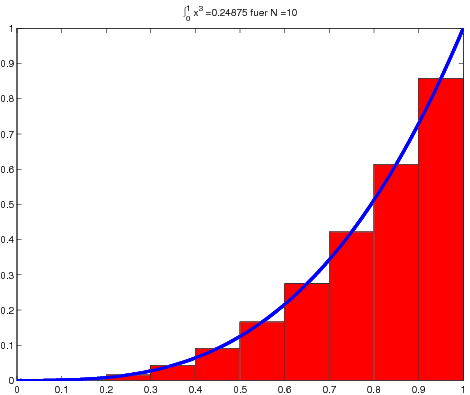
\includegraphics[width=\textwidth]{./../figures/integral_N=10} 
\column{0.5\textwidth}
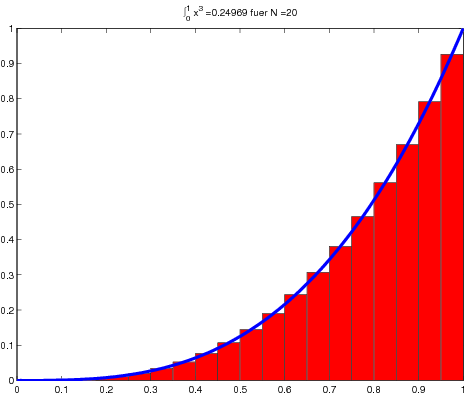
\includegraphics[width=\textwidth]{./../figures/integral_N=20}
\end{columns}
\end{frame}
% 
% Slide
% 
\begin{frame}[fragile]\frametitle{Programm}
\begin{lstlisting}
%   integral.m

N = 20; % Anzahl Unterteilungen

x = (0+1/(2*N)):(1/N):(1-1/(2*N));
y = x.^3;
% Berechnung des Integrals
result = sum(y)*(1/N);

% Plot
for i = 1:N
    fill([(i-1)/N (i-1)/N i/N i/N], ...
      [0 ((i-0.5)/N).^3  ((i-0.5)/N).^3 0], 'r');
    hold on;
end;
plot(0:0.01:1,(0:0.01:1).^3,'LineWidth',3);
title(['\int_0^1 x^3! = ',num2str(result),...
  ' fuer N =', num2str(N)]); 
\end{lstlisting}
\end{frame}

\subsection{Dreidimensionale Grafiken}

% 
% Slide
% 
% 
\begin{frame}[fragile]\frametitle{Dreidimensionale Grafiken}
\begin{itemize}
\item Dreidimensionale Version von \lstinline!plot!: \alert{ \lstinline!plot3!}
\item Darstellung von Funktionen $f:\mathbb{R}^2 \ \rightarrow \
  \mathbb{R}$:
\begin{itemize}
\item Contourplot (zeichnet die Niveaulinien): \alert{ \lstinline!contour!}, \alert{
    \lstinline!contourf!}, \alert{ \lstinline!contour3!}
\item Darstellung des Graphen mit Gitterlinien: \alert{ \lstinline!mesh! ,
  \lstinline!meshc!} 
\item Flächige Darstellung des Graphen: \alert{ \lstinline!surf!, \lstinline!surfc!}
\end{itemize} 
\item Darstellung von Funktionen $f:\mathbb{R}^3 \ \rightarrow \
  \mathbb{R}$:
\begin{itemize}
\item Streifenansichten \alert{ \lstinline!slice!}
\end{itemize}
\end{itemize}
\end{frame}

% 
% Slide
% 
\begin{frame}[fragile]\frametitle{plot3}
Bei gegebenen Vektoren $x=(x_i)_{i=1}^n$, $y=(y_i)_{i=1}^n$,
$z=(z_i)_{i=1}^n$ erzeugt \alert{ \lstinline!plot3(x,y,z)!} einen Plot der die Punkte
$(x_i,y_i,z_i)$ und $(x_{i+1},y_{i+1},z_{i+1})$ miteinander
verbindet. \\
\begin{center}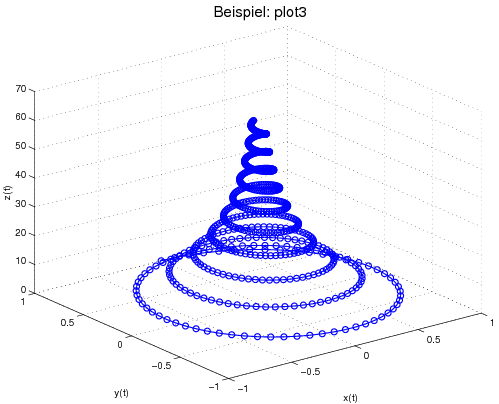
\includegraphics[width=0.6\textwidth]{./../figures/beispiel_plot3}\end{center}
\end{frame}
% 
% Slide
% 
\begin{frame}[fragile]\frametitle{Beispiel plot3}
\begin{lstlisting}
t = 0:0.1:20*pi;
x = exp(-t/20).*sin(t);
y = exp(-t/20).*cos(t);
z = t;

plot3(x,y,z,'b-o','LineWidth',1);
grid on
xlabel('x(t)'), ylabel('y(t)');
 zlabel('z(t)');
title('Beispiel: plot3','FontSize',15);
\end{lstlisting}
\end{frame}
% 
% Slide
% 
\begin{frame}[fragile]\frametitle{Blickwinkel}
\centering\alert{ \lstinline!view(az,el)!}
\begin{itemize}
\item \alert{ \lstinline!az!} ist die horiz. Rotation in Grad (Def. \alert{
  $-37.5$}) 
\item \alert{ \lstinline!el!} ist die vertikale Rotation in Grad (Def. \alert{
  $30$})
\end{itemize}
\begin{center}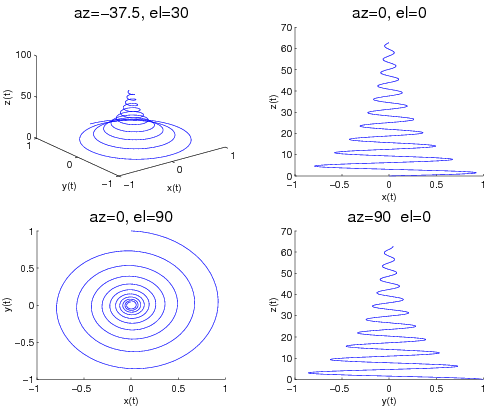
\includegraphics[width=0.6\textwidth]{./../figures/beispiel_plot3_2}\end{center}
\end{frame}
% 
% Slide
% 
\begin{frame}[fragile]\frametitle{3D-Funktionenplots}

Darstellung von Funktionen
\[ f: \mathbb{R}^2 \quad  \rightarrow \quad \mathbb{R} \]
\hspace*{1cm}\\

\textbf{Beispiel:}\\
\alert{ \[ f(x,y):=\exp(-x^2-y^2)\sin(\pi x y) \]}
\end{frame}
% 
% Slide
% 
\begin{frame}[fragile]\frametitle{Beispiel: Funktionenplot}
\hfil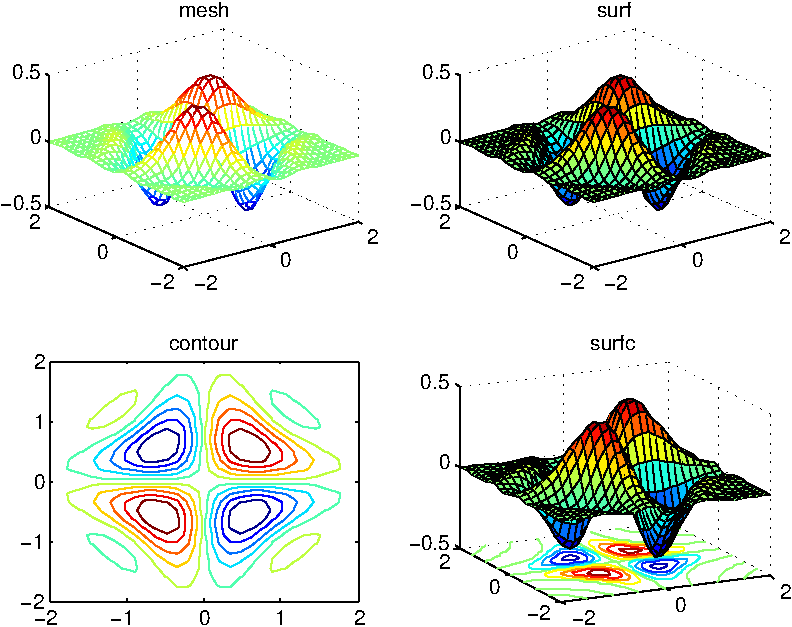
\includegraphics[width=0.8\textwidth]{./../figures/beispiel_function_plot_3d}\hfil
\end{frame}
% 
% Slide
% 
\begin{frame}[fragile]\frametitle{Programm}
\begin{lstlisting}
% Erzeugen des Gitters
x = linspace(-2,2,30);
y = linspace(-2,2,30);
[X,Y] = meshgrid(x,y);
% Funktionswerte
Z = exp(-X.^2-Y.^2).*sin(pi*X.*Y);

% verschiedenen Darstellungen
subplot(2,2,1),
 mesh(X,Y,Z), title('mesh');
subplot(2,2,2),
 surf(X,Y,Z), title('surf');
subplot(2,2,3),
 contour(X,Y,Z,10), title('contour');
subplot(2,2,4),
 surfc(X,Y,Z);
 view(-26,20), title('surfc');
\end{lstlisting}
\end{frame}
% 
% Slide
% 
\begin{frame}[fragile]\frametitle{subplot}
\begin{lstlisting}
subplot(n,m,k),
\end{lstlisting}
zerlegt das Grafikfenster in $n \times m$ Teilfenster. 

Die Zahl $1
\leq k \leq nm$ gibt an, welches Teilfenster gerade aktiv
ist. \\

Durchnumeriert wird zeilenweise, also $(1,1), (1,2), \dots$.

\end{frame}

% 
% Slide
% 
\begin{frame}[fragile]\frametitle{meshgrid}
Zu Vektoren $x=(x_i)_{i=1}^k$, $y=(y_j)_{j=1}^n$ erzeugt 
\begin{lstlisting}
[X,Y]=meshgrid(x,y)
\end{lstlisting}
Matrizen $X,Y \in \mathbb{R}^{n \times k}$, wobei jede Zeile von $X$
eine Kopie des Vektors $x$ ist und $Y$ als Spalten den Vektor $y$
enthält. \\
Dann hat \alert{ \lstinline!Z=X.*Y!} die Komponenten 
\[ Z(i,j)=x(j)*y(i). \]
\end{frame}
% 
% Slide
% 
\begin{frame}[fragile]\frametitle{Darstellungsmöglichkeiten}
\begin{itemize}
\item Contourplot (zeichnet die Niveaulinien): \alert{ \lstinline!contour!}
\item Darstellung des Graphen mit Gitterlinien: \alert{ \lstinline!mesh! ,
  \lstinline!meshc!} 
\item Flächige Darstellung des Graphen: \alert{ \lstinline!surf!, \lstinline!surfc!}
\end{itemize} 

\alert{ \lstinline!mesh(X,Y,Z)!} z.B. stellt für Matrizen $X,Y,Z \in
\mathbb{R}^{n \times k}$ die Punkte 
\[\alert{  (X(i,j), Y(i,j), Z(i,j))} \quad \mbox{dar.}\]
\end{frame}
% 
% Slide
% 
\begin{frame}[fragile]\frametitle{Weitere Möglichkeiten}
\begin{itemize}
\item Darstellung versteckter Linien (bei \lstinline!mesh!): \alert{ \lstinline!hidden off!}, Default:
\alert{ \lstinline!hidden on!}
\item Verschmieren des Gitters: \alert{ \lstinline!shading('interp')!}
\item Blickwinkel: \alert{ \lstinline!view(az,el)!}
\item ähnlich wie \lstinline!mesh!; nur mit 'Vorhang': \alert{
  \lstinline!meshz(X,Y,Z)!}
\end{itemize}
\end{frame}
% 
% Slide
% 
\begin{frame}[fragile]\frametitle{Beispiel: Funktionenplot}
\hfil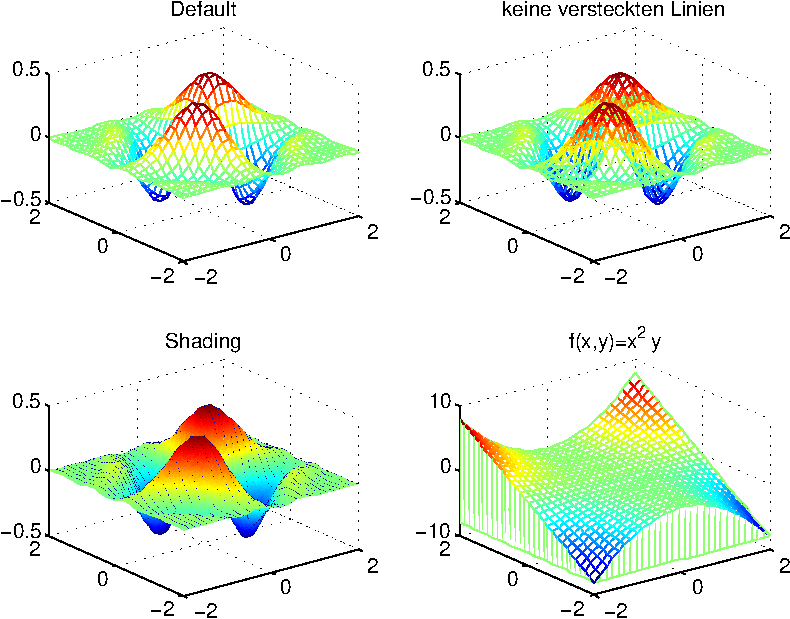
\includegraphics[width=0.8\textwidth]{./../figures/beispiel_function_plot_3d_2}\hfil
\end{frame}
% 
% Slide
% 
\begin{frame}[fragile]\frametitle{Programm}
\begin{lstlisting}
x = linspace(-2,2,30);
y = linspace(-2,2,30);
[X,Y] = meshgrid(x,y);
% Funktionswerte
Z = exp(-X.^2-Y.^2).*sin(pi*X.*Y);

% verschiedenen Darstellungen
subplot(2,2,1),
 mesh(X,Y,Z), title('Default');
subplot(2,2,2),
 mesh(X,Y,Z), hidden off,
 title('keine versteckten Linien');
subplot(2,2,3), surf(X,Y,Z);
 shading('interp'), title('Shading');
subplot(2,2,4), Z=X.^2.*Y;
 meshz(X,Y,Z), title('f(x,y)=x^2 y');
\end{lstlisting}
\end{frame}

% 
% Slide
% 
\begin{frame}[fragile]\frametitle{Contour Plots}
\hfil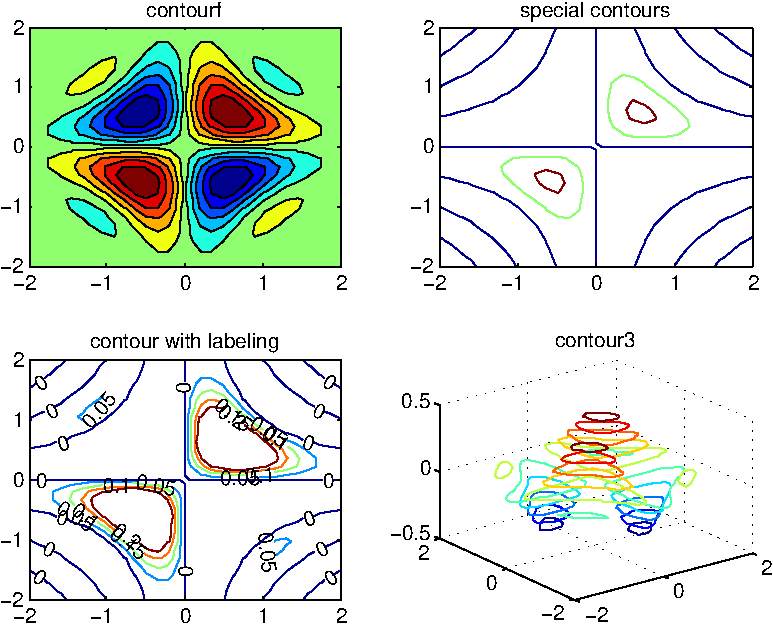
\includegraphics[width=0.8\textwidth]{./../figures/beispiel_function_plot_contour}\hfil
\end{frame}
% 
% Slide
% 
\begin{frame}[fragile]\frametitle{Contour Plots - Listing}
\begin{lstlisting}
% verschiedenen Darstellungen
subplot(2,2,1),
 contourf(X,Y,Z,10), title('contourf')
subplot(2,2,2),
 contour(X,Y,Z,[0 0.2 0.4]), title('special contours');
subplot(2,2,3),
 [C,h] = contour(X,Y,Z,[0 0.05 0.1 0.15 0.2 ]); 
 title('contour with labeling');
 clabel(C,h)
subplot(2,2,4),
  contour3(X,Y,Z,10), title('contour3')
\end{lstlisting}
\end{frame}

% 
% Slide
% 
\begin{frame}[fragile]\frametitle{Erläuterungen zu Contour-Befehlen}
\begin{itemize}
\item \lstinline!contour(X,Y,Z,n)! zeichnet f\"ur $n\in \mathbb{N}$
  $n$-Konturlinien. Ist $n$ ein Vektor, werden Konturlinien zu den Werten in
  dem Vektor $n$ geplottet.
\item \lstinline!contourf! funktioniert wie \lstinline!contour! nur das die Flächen
  zwischen den Konturlinien ausgefüllt werden.
\item \lstinline!label(C,h)! beschriftet die Konturlinien, deren Werte in $C$
  gespeichert sind und die zum Grafik-Handle $h$ gehören.
\item \lstinline!contour3! zeichnet jede Konturlinie auf einer anderen H\"ohe.
\end{itemize}
\end{frame}
%
% Slide
% 
\begin{frame}[fragile]\frametitle{Slice}
\begin{lstlisting}
slice(X,Y,Z,V,sx,sy,sz)
\end{lstlisting}
zeichnet  Schnitte zu den Funktionswerten $V(i)$ zu
$(X(i),Y(i),Z(i))$. Schnitte sind durch die Vektoren $sx$, $sy$ und $sz$
gegeben.\\
\textbf{Beispiel}: \alert{ \[ f(x,y,z):=\exp(-x^2-y^2)\sin(\pi x y z) \]}
\begin{lstlisting}
x = linspace(-2,2,20);
[X,Y,Z] = meshgrid(x,x,x);
V =  exp(-X.^2-Y.^2).*sin(pi*X.*Y.*Z);
sx = [-0.5,0,0.5]; sy = [-1,0,1]; 
sz = [];
slice(X,Y,Z,V,sx,sy,sz)
alpha(0.6) % Transparency
\end{lstlisting}
\end{frame}

\subsection{Animation}
% 
% Slide
% 
\begin{frame}[fragile]\frametitle{Animation-Beispiel}
\begin{lstlisting}
% animation.m

clear all;
[X,Y] = meshgrid(-1:0.05:1,-1:0.05:1);

for j = 1:30
    Z = cos(j^0.5*pi*exp(-X.^2-Y.^2));
    mesh(X,Y,Z);
    F(j) = getframe;
end
% Abspielen des Movies
movie(F,1);
\end{lstlisting}
\end{frame}
%
% Slide
% 
\begin{frame}[fragile]\frametitle{Erstellen einer Animation}
\begin{itemize}
\item Mit \lstinline!F(j)=getframe! wird die aktuelle Grafik in das Array
  $F$ gespeichert.
\item Nach dem alle Bilder zu $F$ hinzugefügt worden sind, kann man
  die Sequenz der Bilder $F$ darstellen durch \lstinline!movie(F,n,fps)!,
  wobei $n$ die Anzahl der Wiederholungen angibt und $fps$ der
  gezeigten Frames pro Sekunde entspricht (Default: $n=1$, $fps=12$). 

\item Speichern des Movies in AVI Format: \lstinline!movie2avi(F,Dateiname)!
\end{itemize}
\end{frame}

%
% Slide
%
\section{Polynome}
\subsection{Interpolation Extrapolation}

%
% Slide
%
\begin{frame}[fragile]\frametitle{Polynome}
In MATLAB werden Polynome
\[ p(x)=p_1 x^n+ p_2 x^{n-1}+ \cdots + p_{n+1} \]
repr\"asentiert durch einen Zeilenvektor $p=[p(1) \ p(2) \ \dots
\   p(n+1)]$. \vspace*{0.5cm}\\

\alert{ Vorsicht:} Normalerweise werden Polynome in der Form
$\sum_{i=0}^n p_ix^i$ dargestellt. In MATLAB dagegen ist die
Darstellung invers und beginnt bei $1$.
\end{frame}
%
% Slide
%
\begin{frame}[fragile]\frametitle{Problemstellungen}
\begin{itemize}
\item [1.] \alert{ Auswerten:} Bei gegebenen Koeffizienten, das
  zugeh\"orige Polynom an bestimmten Stellen auswerten.
\item [2.] \alert{ Nullstellenbestimmung:} Bestimme zu gegebenen
  Koeffizienten die Nullstellen des zugeh\"origen Polynoms.
\item [3.]  \alert{ Interpolation}: Bestimme zu einer gegebenen Menge von
  Punkten $(x_i,y_i)_{i=0}^n$ ein Polynom $n$.-ten Grades, das durch
  diese Punkte verl\"auft.
\end{itemize}
\end{frame}
%
% Slide
%
\begin{frame}[fragile]\frametitle{Auswerten}
Durch 
\begin{lstlisting}
y=polyval(p,x)
\end{lstlisting}
werden aus einem vorgegebenen Koeffizientenvektor $p$ und
entsprechenden Stellen $x$ die zugeh\"origen Funktionswerte $y$
berechnet. $x$ kann eine Matrix sein. $y$ ist dann von der gleichen
Dimens. wie $x$.\\[0.2cm]

\alert{Beispiel:} $p(x):= x^3 - x^2 +1$\\
\begin{columns}[c]
\column{0.55\textwidth}
\begin{lstlisting}
>> x=-2:0.1:2; 
>> y=polyval([1 -1 0 1],x); 
>> plot(x,y,'r--','Linewidth',3);
\end{lstlisting}
\column{0.45\textwidth}
%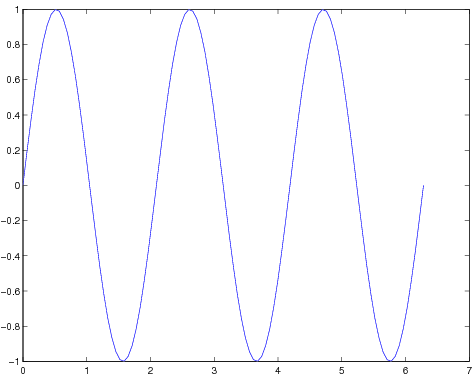
\includegraphics[width=5cm, height=3cm]{grafik_1}
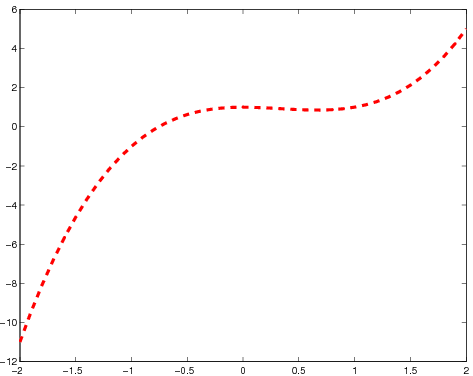
\includegraphics[width=\textwidth]{./../figures/polynom1}
\end{columns}
\end{frame}
%
% Slide
%
\begin{frame}[fragile]\frametitle{Bestimmung von Nullstellen}
Ist $p$ der obige Koeffizientenvektor, so k\"onnen die Nullstellen $z$
durch \lstinline!z = roots(p)! berechnet werden. 

\textbf{Beispiel:} \\
Nullstellen von $p(x):= x^3 - x^2 +1$\\
\begin{columns}[c]
\column{0.56\textwidth}
\begin{lstlisting}
>> roots([1 -1 0 1])
ans =
   0.8774 + 0.7449i
   0.8774 - 0.7449i
  -0.7549  
>> x=-1:0.1:1; [X,Y]=meshgrid(x,x);
>> Z=abs(polyval([1 -1 0 1],X+i*Y)); 
>> surf(X,Y,Z)
\end{lstlisting}
\column{0.45\textwidth}
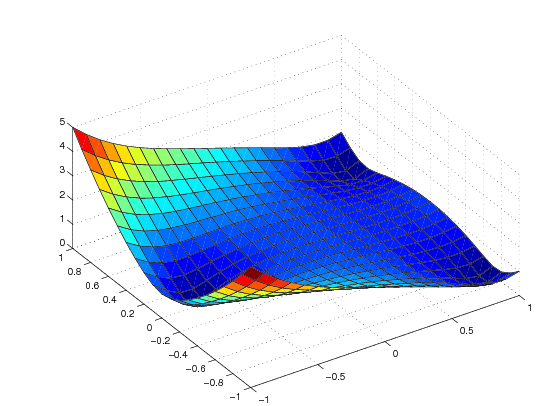
\includegraphics[width=\textwidth]{./../figures/polynom2}
\end{columns}
\end{frame}
% 
% Slide
%
\begin{frame}[fragile]\frametitle{Interpolation}
Suche zu gegebenen Punkten $(x_i,y_i)_{i=0}^n$ ein Polynom $p$
$n$.-ten Grades, so dass $p(x_i)=y_i$ gilt f\"ur $i=0, \dots ,n$.\\
In MATLAB: \alert{ \lstinline!p=polyfit(x,y,n)!} \\[0.5cm]

Ruft man \alert{ \lstinline!p=polyfit(x,y,m)!} mit $m<n$ auf, so sucht MATLAB
die Least Square L\"osung, d.h. das Polynom $p$ der Ordnung $m$,
welches \\
 $\sum_{i=0}^n (p(x_i)-y_i)^2$ minimiert.
\end{frame}

%
% Slide
%
\begin{frame}[fragile]\frametitle{Data Fitting}
Ein weiterer Befehl  zur Interpolation ist
\begin{lstlisting}
yi=interp1(x,y,xi,'method').
\end{lstlisting}
Dabei sind $(x,y)$ die gegebenen Punkte, $xi$ sind die Stellen, an die
die Interpolante berechnet wird und $yi$ sind die entsprechenden
Funktionswerte. 
Als \lstinline!'method'! gibt es\\

{\scriptsize
\begin{tabular}{ll}
'nearest' &  stückweise konstante Approximation \\
'linear'  & Lineare Interpolation \\ 
'spline' & stückweise kubischer Spline $u$ ($u \in C^2$,
$u|_{[x_i,x_{i+1}]} \in \mathbb{P}_3$) \\
'cubic' & kubische Hermite Interpolation\\ 
\end{tabular}
}
\end{frame}
%
% Slide
%
\begin{frame}[fragile]\frametitle{Beispiel}
\hfil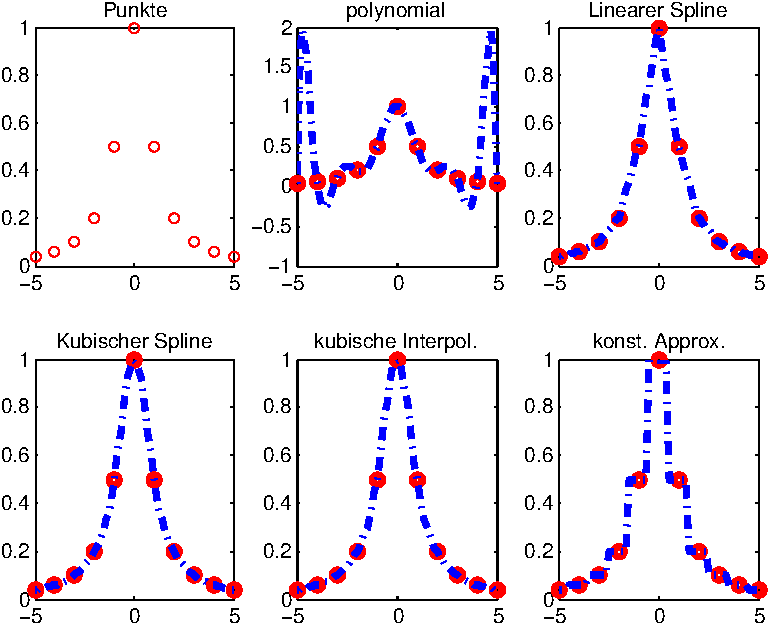
\includegraphics[width=0.8\textwidth]{./../figures/data_fitting}\hfil
\end{frame}
%
% Slide
%
\begin{frame}[fragile]\frametitle{Bemerkungen}
\begin{itemize}
\item  Nur für die Spline-Methoden können   bei \lstinline!interp1!  auch
  Stellen außerhalb des
  Interpolationsintervalls berechnet werden.
\item Data Fitting kann auch über die Oberfläche durchgeführt werden.
 Plotten Sie die Daten und wählen Sie \lstinline!Basic Fitting! im Men\"u
 \lstinline!Tools!. 
\end{itemize}
\end{frame}
%
% Slide
% 
\begin{frame}[fragile]\frametitle{Lineare Regression}
\begin{lstlisting}
% Example for Linear Regression 
x = (1:0.5:4)';
y = exp(x);
plot(x,y,'o');
hold on;
pause;
%--- Determine least square fit for

%    f(t)=a(1) + a(2) t + a(3) t^2

n=length(x);
A = [ ones(n,1), x, x.^2 ];
a = A \ y;
%--- Plot new curve
x1 = 1:0.1:4;
y1 = a(1) + a(2)*x1 + a(3)*x1.^2;
plot(x1,y1,'LineWidth',2)
\end{lstlisting}
\end{frame}

\end{document}




